\section{Úvod}
\label{chap:introduction}

Tato příručka slouží jako pomůcka pro vývojáře, kteří chtějí vyvíjet grafické uživatelské rozhraní (GUI). Budeme se soustředit na rozhraní webových stránek, ale některé zásady lze aplikovat pro jakékoliv GUI.

V~první části se seznámíme s~technologiemi, které se používají pro vývoj GUI. Řekneme si několik základních principů, které bychom měli dodržovat při vývoji GUI. Popíšeme si postup, který můžeme využít při návrhu a~vývoji GUI. Obsah příručky je také doplněn o~konkrétní příklady z~vývoje mé bakalářské práce, které ukazují použití některých bodů v~praxi.

\section{Zásady vývoje webového GUI}
\label{sec:principles}

Pro uživatelsky přívětivé GUI je důležité dodržovat několik zásad. Ty jsou založeny na praktických zkušenostech grafiků a~psychologických studiích. Nyní se podíváme na základní principy, které by mělo moderní uživatelské rozhraní splňovat. V~krátkosti si představíme několik z~nich.

\subsection{Vzhled stránky}
\label{subsec:visual-principles}

\begin{itemize}
  \item \textbf{Kontrast} -- Je jedním z~nejdůležitějších prvků designu. Zajišťuje, že text a~další prvky jsou čitelné a~viditelné. Je důležitý pro umocnění dojmu a~pro zvýraznění důležitých prvků.
  \item \textbf{Vyváženost} -- Všechny prvky na stránce mají pomyslnou váhu, která je dána jejich velikostí, barvou, kontrastem a~dalšími faktory. Zajišťuje, že tyto prvky jsou rozloženy tak, aby stránka působila vyváženě a~přehledně.
  \item \textbf{Důraz} -- Slouží pro zvýraznění důležitých prvků a~k~pomyslnému ukrytí těch méně podstatných. Můžeme tak ovládat výraznost jistých informací a~zároveň usměrňovat pozornost uživatele.
  \item \textbf{Proporce} -- Správně určené proporce podporují výše zmíněnou vyváženost. Pomáhají uživateli orientovat se na stránce a~zároveň zajišťují, že stránka působí přehledně a~esteticky.
  \item \textbf{Hierarchie} -- Je klíčová pro zdůraznění důležitých prvků v~designu. Tento princip se často projevuje skrze tituly a~nadpisy, které indikují jejich význam ve vztahu k~ostatním prvkům a~obsahu stránky.
  \item \textbf{Opakování} -- Je účinný nástroj pro sjednocení myšlenek v~rámci designu. Konzistentní používání barev, písem, tvarů a~dalších prvků pomáhá sjednotit vzhled stránky.
  \item \textbf{Rytmus} -- Určuje uspořádání prvků na stránce, což může vzbuzovat dojem uspořádanosti nebo naopak chaotičnosti.
  \item \textbf{Vzory} -- Používání vzorů v~designu vytváří pocit předvídatelnosti a~pohodlí pro uživatele.
  \item \textbf{Volný prostor} -- Volný prostor mezi prvky na stránce pomáhá zvýraznit ty důležité a~zajišťuje, že stránka není přeplněná.
  \item \textbf{Navigace pohledem} -- Správná aplikace předešlých principů umožňuje uživateli snadnou a~pohodlnou navigaci po stránce.
  \item \textbf{Rozmanitost} -- Na rozdíl od předešlých bodů, rozmanitost nenapomáhá orientaci na stránce, ale zajišťuje, aby byla pro uživatele zajímavá.
  \item \textbf{Spojitost} -- Spojuje prvky na stránce dohromady, často pomocí opakování barev nebo minimálního počtu fontů.
\end{itemize}

\begin{figure}[H]
  \centering
  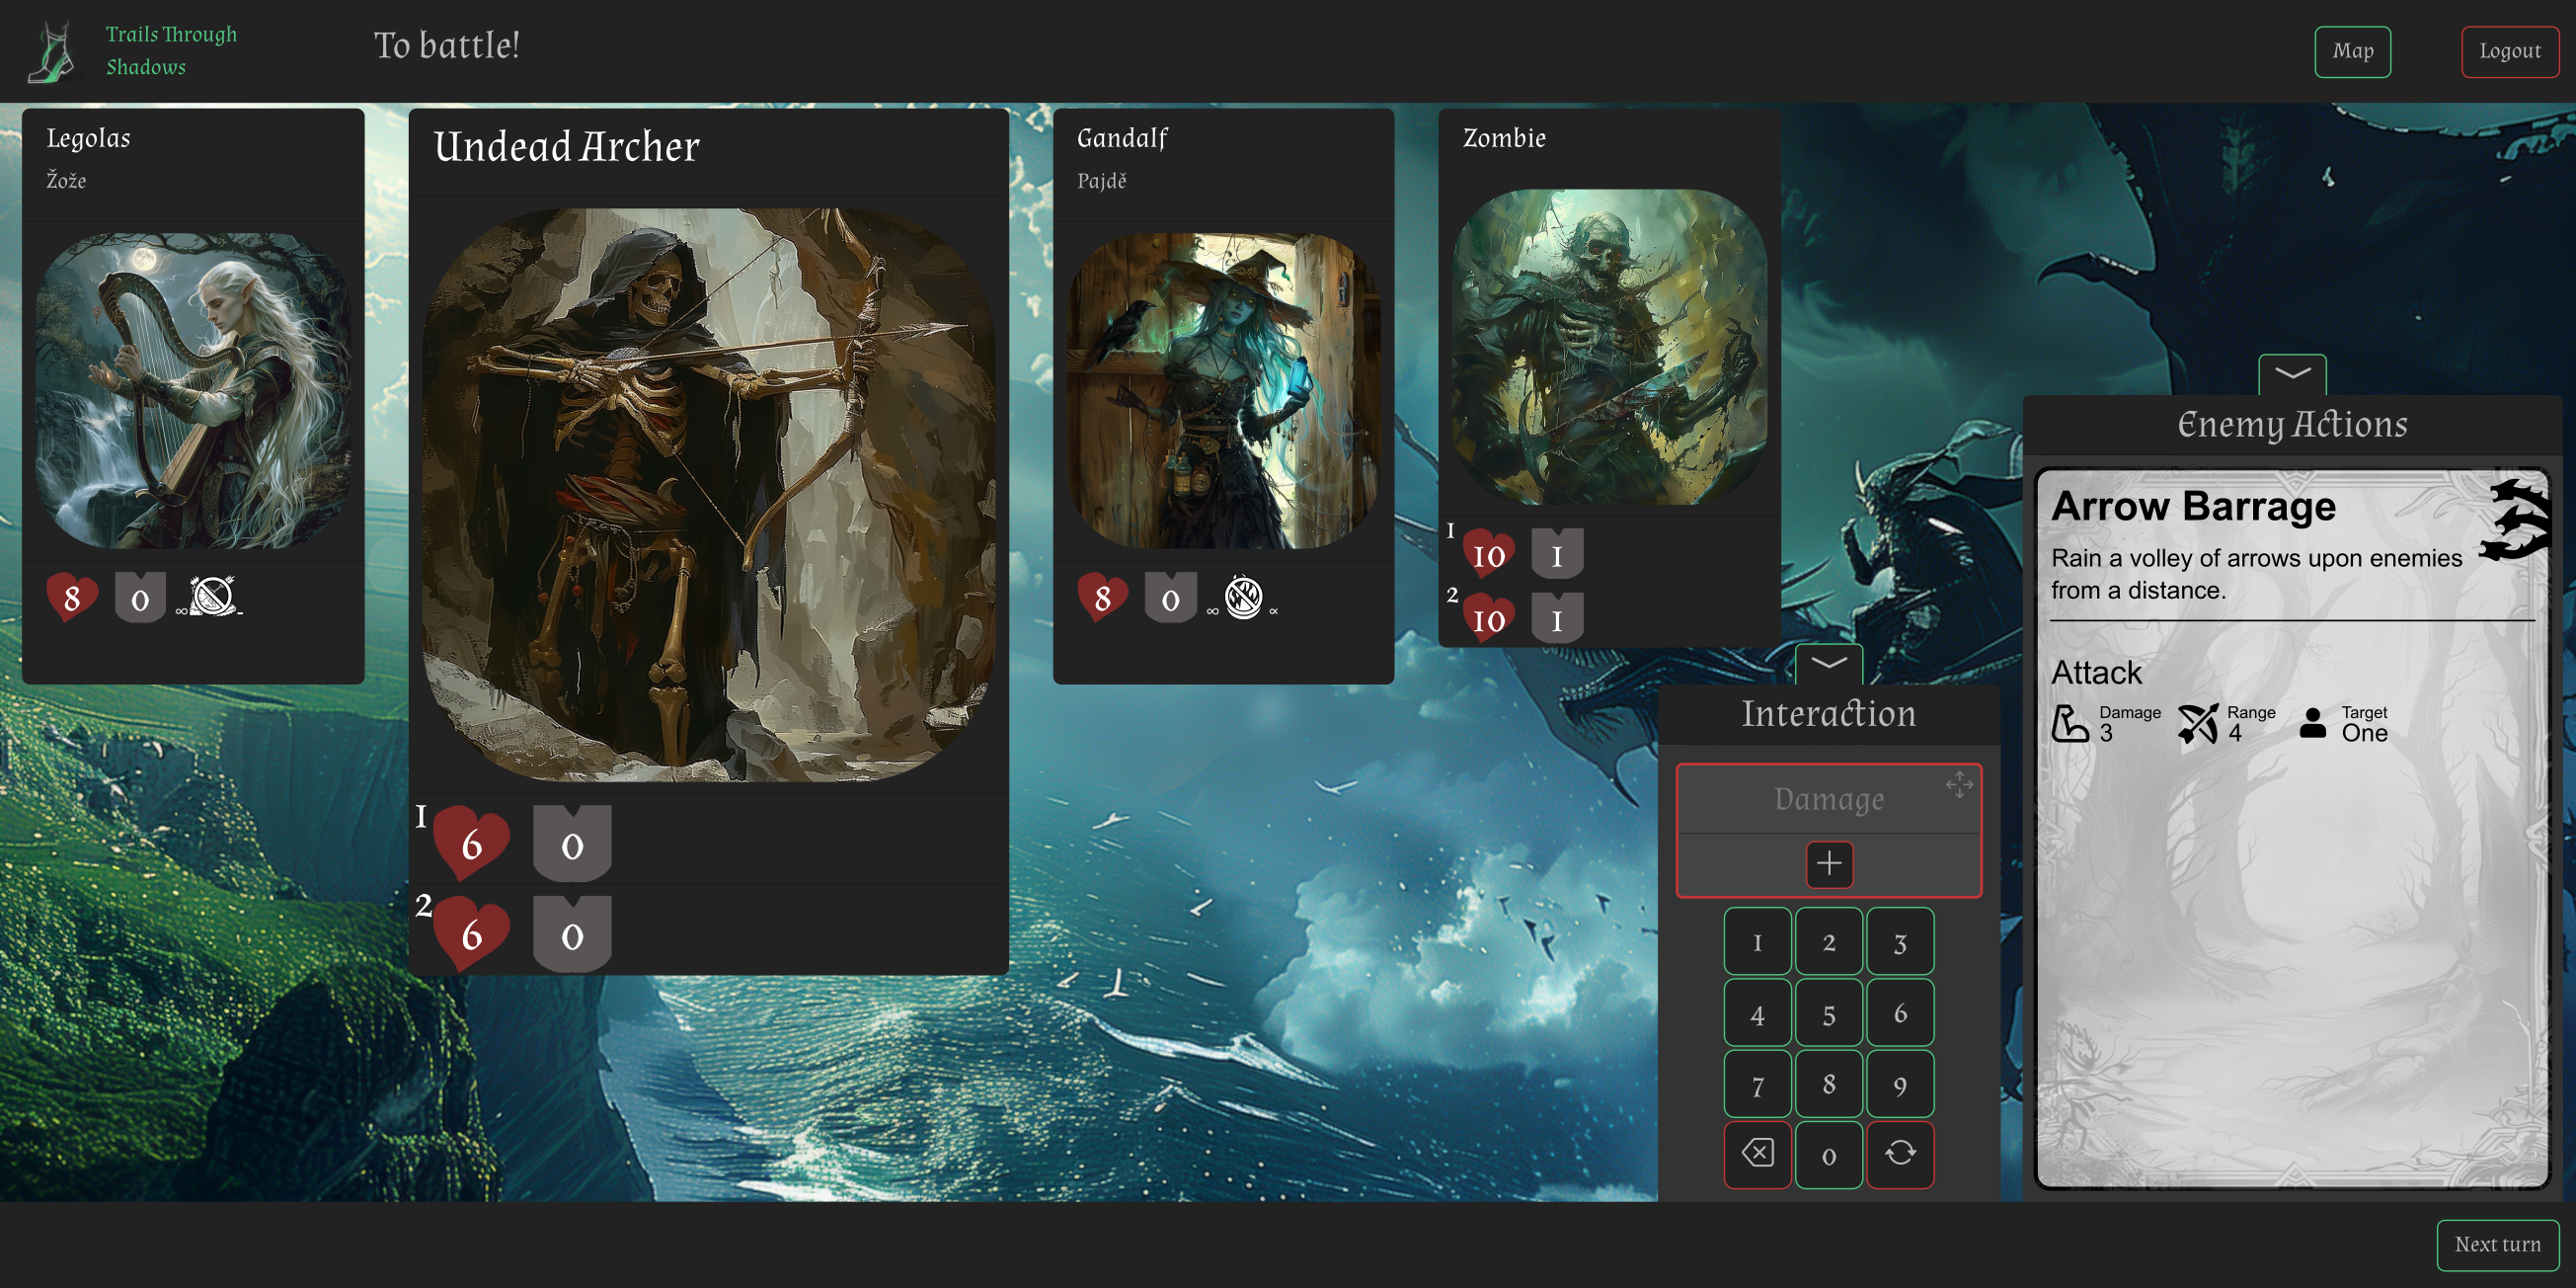
\includegraphics[width=\textwidth]{resources/figures/example1.png}
  \caption{Ukázka z~aplikace 1}
  \label{fig:example1}
\end{figure}

\textit{Na obrázku výše si můžeme znázornit několik z~těchto principů. Jedná se o~ukázku střetnutí, na které můžeme vidět karty entit s~ukazately životů, obrany a~efektů. Dále je na pravé straně znázorněna kartička akce a~vedle ní se nachází panel pro uživatelské vstupy. Karta entity, která je zrovna na tahu je zvětšená, což zajišťuje důraz. Karty jsou uspořádány do řady, což podporuje rytmus. Důraz je zajištěn světlým textem na tmavém pozadí (nebo naopak v~případě akce). Pozadí stránky je také dostatečné světlé aby umocňovalo kontrast s~tmavými kartami. Všechny karty mají stejný formát (opakování), ale zároveň mají každá jiný obrázek (rozmanitost). Tlačítka na vstupím panelu evokují známý design, který lze najít například na klávesnici telefonů (vzory). Všechny tyto prvky dohromady tvoří jednotný design, který je přehledný a~estetický.}

\subsubsection{Teorie barev}
Výběr barev je klíčovým prvkem designu uživatelského rozhraní. Teorie barev zkoumá vztahy mezi barvami a~jejich psychologickými a~emocionálními účinky. Správné použití barev může ovlivnit uživatelovo vnímání aplikace.

Barvy se člení na teplé a~studené. Teplé barvy, jako jsou červená, oranžová a~žlutá, patří do části spektra, která často evokuje radost a~energii. Studené barvy, jako jsou zelená, modrá a~fialová, zase často přinášejí pocit klidu a~harmonie. Volba mezi teplými a~studenými barvami může ovlivnit celkový dojem, který uživatel získá z~aplikace.

\subsubsection*{Barevný kruh}
Často používá díky jeho intuitivnímu rozložení barev. Obsahuje všechny barvy, které lze vytvořit smícháním tří primárních barev a~díky přidání černé či bílé barvy umožňuje i~úpravu jejich odstínů. Existuje několik způsobů, jak za pomoci tohoto kruhu barevnou paletu vybrat. Všechny jsou pro lepší přehlednost ukázány na obrázku pod tímto odstavcem.

\begin{itemize}
    \item \textbf{Komplementární}: Barvy, které jsou na opačných stranách kruhu. Při jejich kombinaci vzniká kontrastní efekt.
    \item \textbf{Monochromatické}: Jedná se o~sadu odstínů jedné barvy. Vytváří harmonický efekt.
    \item \textbf{Analogické}: Barvy, které jsou vedle sebe na kruhu. Vytváří přirozený a~pohodlný efekt, ale je vhodné vybrat jednu z~barev jako hlavní a~zbytek používat pouze jako akcenty.
    \item \textbf{Triadické}: Kombinace tří barev, které na kruhu tvoří rovnostranný trojúhelník. Podobně jako způsob komplementární, také vytváří kontrastní efekt.
    \item \textbf{Rozštěpená komplementární}: Variace komplementární kombinace, kde se namísto protější barvy, používají barvy s~ní sousedící. 
    \item \textbf{Tetradické}: Čtyři barvy, kde každé dvě tvoří komplementární pár a~vytvářejí obdélník na barevném kruhu. Vytváří kontrastní efekt, ale zároveň je možné vytvořit i~harmonický efekt, pokud se barvy správně kombinují.
\end{itemize}

\begin{figure}[H]
    \centering
    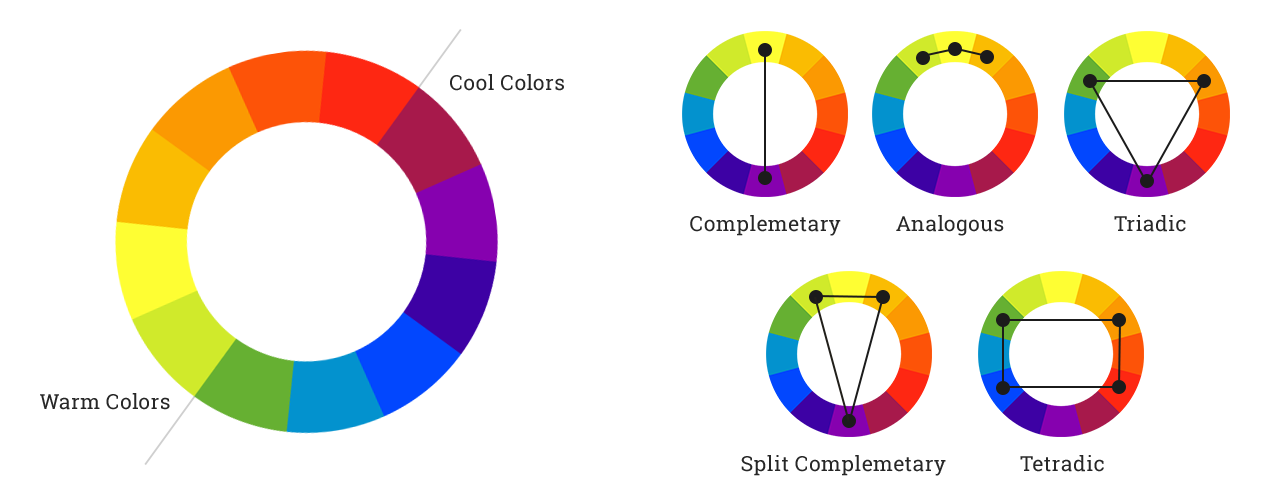
\includegraphics[width=\textwidth]{resources/figures/color_theory.png}
    \caption[Barevný kruh]{Barevný kruh\footnotemark}
    \label{fig:color-wheel}
\end{figure}

\footnotetext{Zdroj:\url{https://www.webascender.com/blog/understanding-color-schemes-choosing-colors-for-your-website}}

\subsubsection{Typografie}
Typografie je umění používání písma a~fontů k~tomu, aby byl text čitelný, srozumitelný a~příjemný ke čtení. Hraje klíčovou roli v~designu UI tím, že ovlivňuje rozpoznatelnost značky, rozhodování a~pozornost uživatele. Dobrá typografie pomáhá při předávání informací a~integruje se s~ostatními prvky rozhraní, zlepšujíc celkovou vizuální rovnováhu a~uživatelskou zkušenost.

\subsection{Použitelnost}
Úzce souvisí se vzhledem stránky a~často se tato témata překrývají, ale zároveň je to samostatný princip, který je nutno uvést zvlášť. Zahrnuje všechny aspekty, které napomáhají uživateli k~snadnějšímu a~pohodlnějšímu užívání stránky. Například:

\begin{itemize}
  \item \textbf{Konzistence} -- Je klíčová pro uživatelskou přívětivost. Uživatelé se rychleji naučí, jak stránka funguje, pokud je konzistentní. To znamená, že by vývojář měl dodržovat stejné rozložení a~navigaci mezi jednotlivými stránkami.
  \item \textbf{Zkratky} -- Mohou urychlit a~tím zpříjemnit uživatelův pohyb po stránce. Tohoto výsledku můžeme dosáhnout například využitím odkazů v~menu či přesměrováním díky kliknutí na logo. Takovéto zkratky by měly být intuitivní a~měly by vycházet z~již známých vzorů.
  \item \textbf{Zpětná vazba} -- Je důležitá, aby uživatel věděl, zda se akce, kterou chtěl provést, povedla či nikoliv, nebo jestli je možnost na nějaký prvek stránky kliknout. Tohoto dosáhneme pomocí animací, změny barvy či zvýraznění.
  \item \textbf{Uzavření dialogu} -- Podstatné pro uživatele, aby věděl, že jeho akce byla úspěšná a~může přejít k~dalšímu kroku. Tohoto můžeme dosáhnout například přesměrováním na jinou stránku či zobrazením dialogu, který uživateli potvrdí, že jeho akce byla úspěšná.
  \item \textbf{Prevence chyb} -- Zabezpečení proti nesprávným vstupům z~uživatelovy strany je podstatné pro předejití zbytečných chyb, které by mohly vést k~frustraci. K~tomuto přispějeme například tím, že nebudeme uživateli dovolovat zadávat písmena do pole, které by mělo obsahovat pouze čísla. Pokud už chyba nenávratně nastane, je důležité uživatele informovat o~tom, co se stalo a~jak ji může napravit.
  \item \textbf{Možnost vrácení} -- Pokud se uživatel rozmyslí či udělá chybu, měl by mít možnost svou akci jednoduše zrušit a~vrátit se do předešlého stavu stránky.
  \item \textbf{Locus of control} -- Tento fenomén by se dal volně přeložit jako těžiště řízení. Uživatelé chtějí mít pocit, že aplikaci řídí a~že rozhraní reaguje na jejich akce. Takového pocitu můžeme dosáhnout tím, že se zeptáme na potvrzení nějaké akce, například odchodu ze stránky s~neuloženými daty. Tím uživateli dáme pocit větší kontroly.
  \item \textbf{Minimalizace nároků na uživatele} -- Klíčová zásada pro uživatelské rozhraní je minimalizace kognitivní zátěže. Kognitivní zátěž může snížit uživatelovu schopnost vykonávat důležité úkoly, proto je důležité, aby počítače převzaly co nejvíce úkonů na sebe. Uživateli můžeme vypomoci třeba zapamatováním si jeho přihlašovacích či osobních údajů, aby je nemusel zadávat při každém přihlášení. Při návrhu bychom měli vždy dávat přednost rozpoznání před vzpomínáním, abychom uživatelům umožnili rychle a~bez problémů dokončit své úkoly.
  \item \textbf{Responzivnost} -- Jedna z~nejdůležitějších vlastností moderního GUI. Responzivní design zajišťuje, že stránka bude vypadat dobře na všech zařízeních, od mobilních telefonů až po stolní počítače, a~to pomocí změny velikosti, schování či přesunutí prvků na stránce. K~tomu se využívají vlastnosti jazyka CSS, nejčastěji media queries, které umožňují nastavit různé styly pro různé velikosti obrazovek. Responzivní design je v~dnešní době kriticky potřebný, protože většina uživatelů používá k~prohlížení internetu mobilní zařízení a~je důležité, aby se jim stránka zobrazila správně a~byla snadno použitelná.
\end{itemize}

Opět budou následovat příklady z~aplikace pro Trails Through Shadows. Některé z~nich lze jen těžko zobrazit staticky, ale pokusím se je alespoň popsat. Konzistence mezi jednotlivými stránkami aplikace je udržována stálou přítomností navigačního menu s~logem v~horní části stránky. Tam kde to jde a~dává smysl je taky přidáno spodní menu, které uchovává tlačítka pro nejčastější akce. Kliknutím na logo se samozřejmě uživatel vrátí na úvodní stránku.

\begin{figure}[H]
  \begin{minipage}{0.35\textwidth}
    \centering
    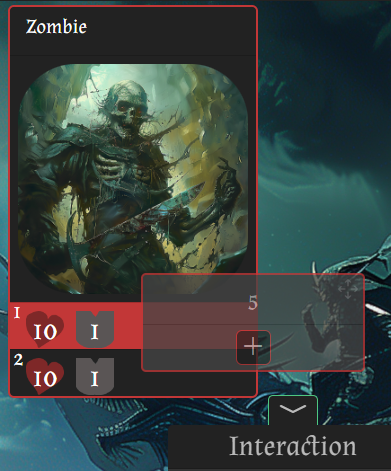
\includegraphics[width=0.9\textwidth]{resources/figures/example2.png}
    \caption{Ukázka zpětné vazby}
    \label{fig:example4}
  \end{minipage}
  \begin{minipage}{0.65\textwidth}
    \centering
    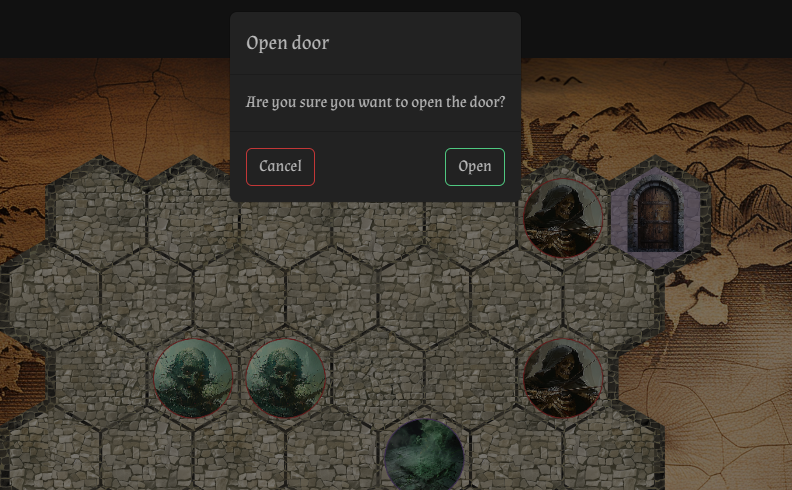
\includegraphics[width=0.9\textwidth]{resources/figures/example3.png}
    \caption{Ukázka těžiště řízení}
    \label{fig:example3}
  \end{minipage}
\end{figure}

\textit{Na obrázku vlevo nahoře můžeme vidět ukázku zpětné vazby při vybírání cíle útoku. Při přetáhnutí ukazatele zranění na cíl, se mu změní barva aby bylo jasné vidět, kdo je zacílen. Na pravém horním obrázku je pak ukázka těžiště řízení, kdy se systém ptá, zda si je uživatel jist otevíráním dveří. Na spodních obrázcích pak můžeme vidět příklad responzivního designu.}

\begin{figure}[H]
  \begin{minipage}{0.3\textwidth}
    \centering
    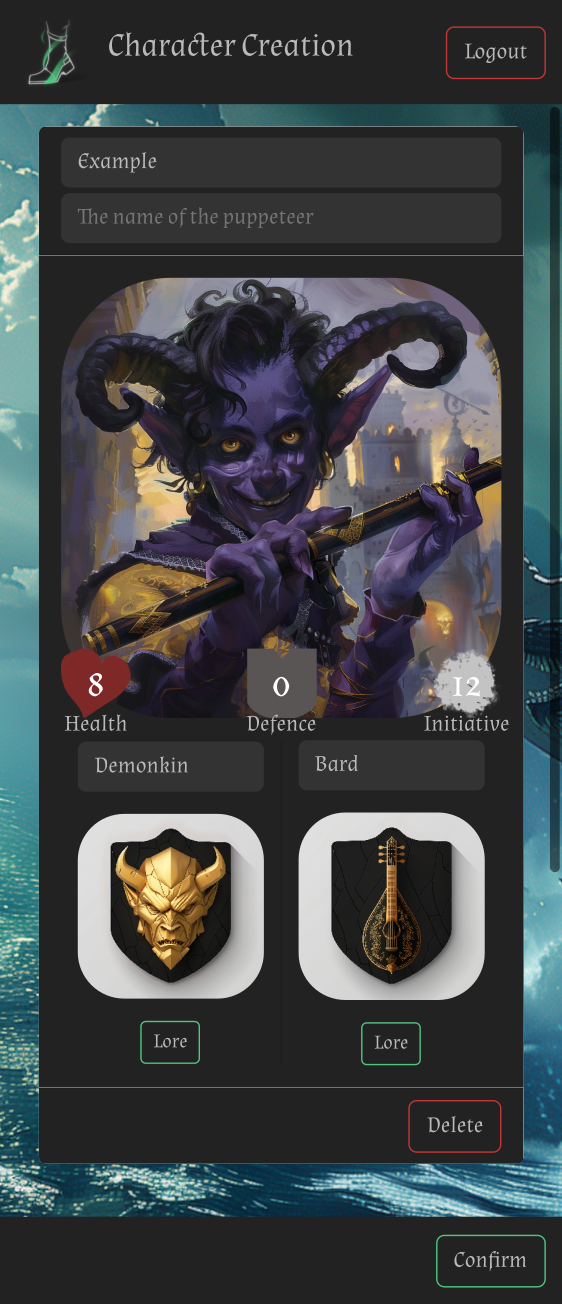
\includegraphics[width=0.9\textwidth]{resources/figures/example5.png}
    \label{fig:example5}
  \end{minipage}
  \begin{minipage}{0.7\textwidth}
    \centering
    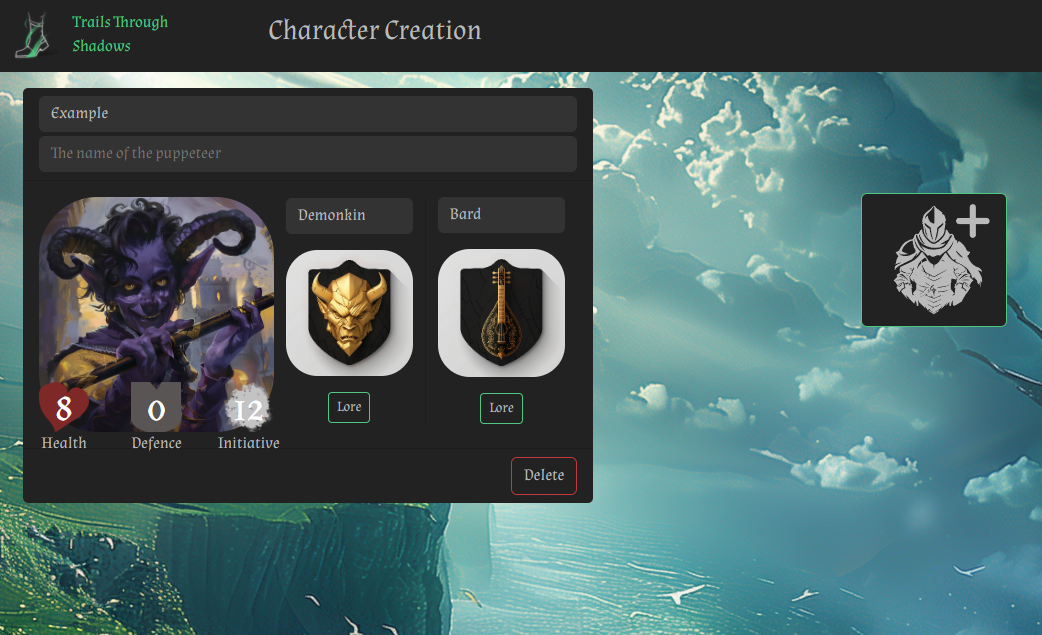
\includegraphics[width=0.9\textwidth]{resources/figures/example6.png}
    \label{fig:example6}
  \end{minipage}
  \caption{Ukázka responzivního designu}
\end{figure}

\section{Technologie}
\label{sec:technologies}

Pro vývoj webových GUI se používají různé technologie. Většina z~nich je založena na jazycích HTML, CSS a~JavaScript. HTML určuje strukturu stránky. Jedná se o~značkovací jazyk, díky kterému jsme schopni definovat jednotlivé elementy na stránce. CSS se používá pro definici vzhledu stránky. Pomocí CSS můžeme měnit barvy, velikosti písma, zarovnání a~mnoho dalších vlastností. JavaScript je skriptovací jazyk, který se používá pro interaktivitu stránky. S~jeho pomocí můžeme měnit obsah stránky v~reálném čase, reagovat na uživatelské akce a~mnoho dalšího.

\subsection{Frameworky}
\label{subsec:frameworks}

Pro vývoj webových aplikací se používají různé frameworky a~knihovny. Několik z~nich bych zde rád uvedl jako přiklady. React je knihovna vyvinutá společností Meta. Angular je framework vyvinutý společností Google. Svelte je kompilátor, který převádí kód napsaný ve Svelte syntaxi na čistý JavaScript. Tyto technologie si nyní v~rychlosti představíme. Který z~nich, pokud nějaký, si vyberete, záleží na vašich preferencích a~potřebách projektu.

\subsection*{React}
\label{subsec:react}

React je knihovna vyvinutá společností Meta (bývalý Facebook). Jedná se o~jednu z~nejpopulárnějších knihoven pro vývoj jednostránkových webových aplikací. Jde o~komponentový framework, což znamená, že celý kód je rozdělen do menších celků zvaných komponenty. Ty jsou znovupoužitelné a~modulární. Mohou být do sebe vnořeny, což nám umožňuje vytvářet složitější struktury. Navíc používá JSX syntaxi, která umožňuje psát HTML kód přímo v~JavaScriptu. Díky tomu je kód lépe čitelný a~snadno se s~ním pracuje. React je znám svou komunitou a~ekosystémem, který je kolem něj postavený. Díky tomu je možné najít spoustu předpřipravených komponent a~knihoven, které urychlí vývoj aplikace. Nedoporučil bych ho však začátečníkům, protože má poměrně strmou křivku učení.

\subsection*{Angular}
\label{subsec:angular}

Angular je framework vyvinutý společností Google. Jedná se o~jednostránkový framework, který je postaven na jazyce TypeScript. TypeScript je nadstavba JavaScriptu, která přidává statické typování a~je striktnější co se týče syntaxe. Díky tomu je kód bezpečnější a~méně náchylný k~chybám. Angular je taktéž komponentový framework. Také má velkou komunitu a~ekosystém, ale je méně populární než React. Je vhodný pro větší projekty, kde je potřeba striktního řízení stavu aplikace.

\pagebreak
\subsection*{Svelte}
\label{subsec:svelte}

Svelte je kompilátor, který převádí kód napsaný ve Svelte syntaxi na čistý JavaScript. Jedná se o~nový přístup k~vývoji webových aplikací. Svelte je komponentový framework, ale na rozdíl od Reactu a~Angularu, kde jsou komponenty interpretovány za běhu, jsou komponenty ve Svelte přeloženy do čistého JavaScriptu. Díky tomu je výsledný kód menší a~rychlejší. Není zdaleka tak populární jako React nebo Angular, ale to nahrazuje svou jednoduchostí a~rychlostí. Svelte je velmi přívětivý na naučení a~je vhodný pro začátečníky.

\begin{figure}[H]
  \begin{minipage}{0.25\textwidth}
    \centering
    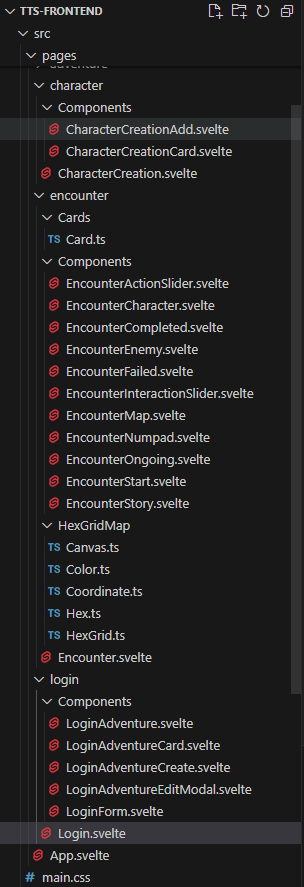
\includegraphics[width=\textwidth]{resources/figures/example7.png}
    \caption{Ukázka složkové struktury}
    \label{fig:example7}
  \end{minipage}
    \begin{minipage}{0.75\textwidth}
    \centering
    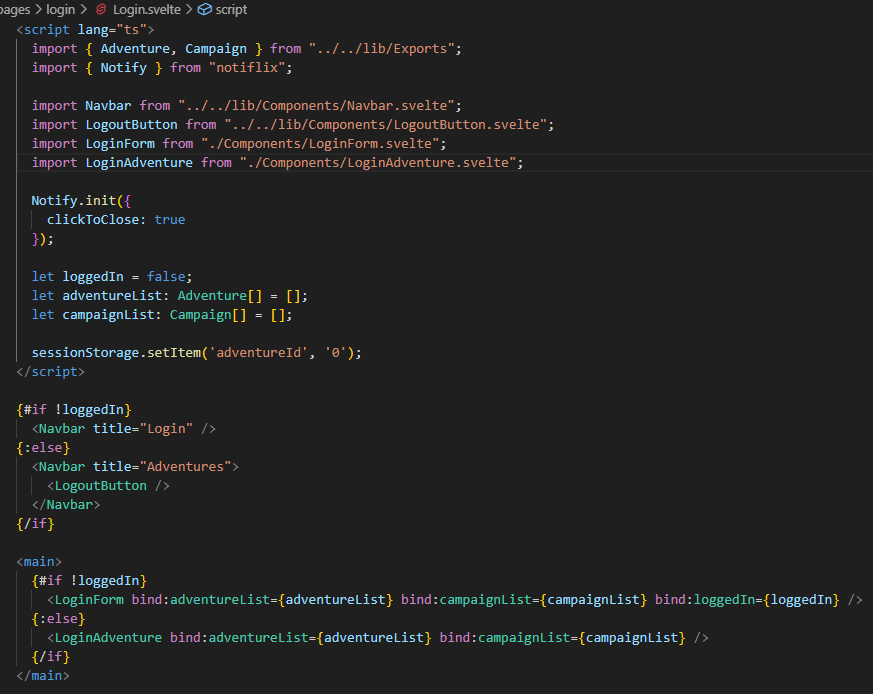
\includegraphics[width=\textwidth]{resources/figures/example8.png}
    \caption{Ukázka Svelte komponenty}
    \label{fig:frameworks}
  \end{minipage}
\end{figure}

\textit{Pro práci na Trails Through Shadows jsem zvolil Svelte. Stalo se tak hlavně kvůli jeho jednoduchosti a~rychlosti. Na obrázku vlevo můžeme vidět složkovou strukturu projektu. Každá složka obsahuje jednu hlavní komponentu a~podsložku s~několika dalšími, které jsou v~ní použity. Na pravém obrázku pak můžeme vidět ukázku Svelte komponenty. Jedná se o~jednoduchou komponentu, která se stará o~zobrazení přihlašovacího formuláře a~hlavní stránky. Všechny komponenty jsou napsány v~Svelte syntaxi, která je velmi intuitivní a~podobná HTML a~CSS, což zjednodušuje práci s~nimi.}

\subsection{Další knihovny}
\label{sec:other-libraries}

Kromě zmíněných frameworků existuje spousta dalších knihoven, které mohou usnadnit vývoj webových aplikací. Slouží jako stavební kameny pro vytvoření jednolitého vzhledu aplikace. Několik takových možností bych zde opět rád uvedl.

\subsection*{Bootstrap}
\label{subsec:bootstrap}

Bootstrap je nejpopulárnější knihovna pro vývoj responzivních webových stránek. Jedná se o~sadu CSS a~JavaScript komponent, které usnadňují jejich tvorbu. Obsahuje mnoho předpřipravených komponent, jako jsou tlačítka, formuláře, navigace a~mnoho dalších. Díky tomu je možné rychle vytvořit moderní a~responzivní webové stránky. Bootstrap lze teoreticky přizpůsobit vlastními CSS styly a~třídami, avšak to může být složité a~velmi rychle se může stát nepřehledným. V~případě, že se chcete vyhnout vlastnímu designu a~pouze potřebujete rychle vytvořit stránku, je Bootstrap ideální volbou. Pokud však chcete vytvořit unikátní design, může být lepší zvolit jinou cestu.

\subsection*{Tailwind CSS}
\label{subsec:tailwind-css}

Tailwind CSS je nový přístup k~psaní CSS. Namísto psaní vlastních CSS stylů, používáme třídy, které definují jednotlivé vlastnosti. Tailwind CSS je velmi flexibilní a~umožňuje vytvářet velkou řadu stylů poměrně jednoduše. Je vhodný pro vývoj moderních a~responzivních webových stránek. Jeho nevýhodou může být velké množství tříd, které je potřeba použít, což může vést k~nepřehlednosti kódu.

\subsection*{Knihovny specifické pro frameworky}
\label{subsec:framework-specific-libraries}

Pro každý z~frameworků existuje spousta takovýchto knihoven. Například pro React existuje Material-UI, React Bootstrap, Ant Design a~mnoho dalších. Tyto knihovny obsahují předpřipravené komponenty, které můžeme použít ve svých aplikacích. Často jsou navrženy tak, aby byly snadno přizpůsobitelné a~rozšiřitelné, ale to se liší od knihovny k~knihovně. Pokud používáte některý z~frameworků, může být užitečné si nějakou takovouto knihovnu najít.

\begin{figure}[H]
  \centering
  \begin{minipage}{0.4\textwidth}
    \centering
    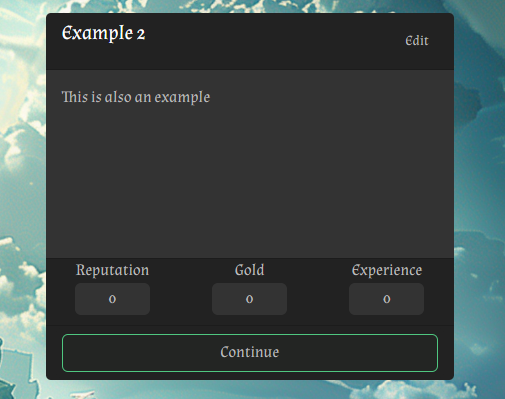
\includegraphics[width=0.9\textwidth]{resources/figures/example9.png}
    \label{fig:example9}
  \end{minipage}
  \begin{minipage}{0.5\textwidth}
    \centering
    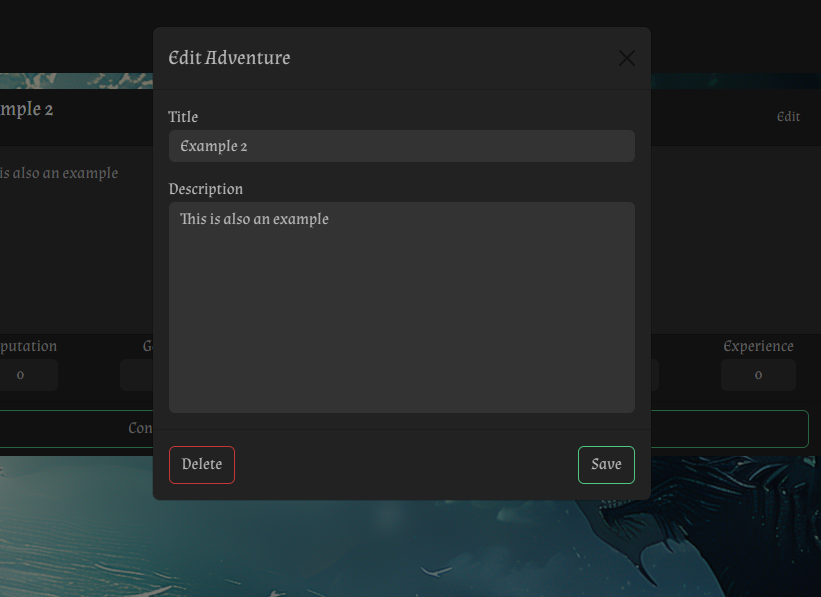
\includegraphics[width=0.9\textwidth]{resources/figures/example10.png}
    \label{fig:example10}
  \end{minipage}
  \caption{Ukázka Bootstrap komponent}
\end{figure}

\textit{Na obrázcích na minulé straně můžeme vidět ukázku Bootstrap komponent. Na levém je komponent karta, na které jsou tlačítka a~textová pole. Na pravém je ukázka modalového okna. Téměř všechny komponenty, které jsem zatím na ukázkách použil, jsou vytvořeny pomocí Bootstrapu: navigace, tlačítka, karty, modální okna a~další. Bootstrap je velmi jednoduchý na použití a~rychle se s~ním pracuje. Jeho nevýhodou může být, že všechny stránky, které jsou vytvořeny pomocí Bootstrapu, vypadají velmi podobně. Zároveň bych chtěl říct, že kdybych projekt dělal znovu, tak si nejspíše vyberu Tailwind CSS, který nabízí větší flexibilitu a~kontrolu nad vzhledem stránky.}

\section{Návrh a~vývoj}
\label{sec:design-and-development}

Nyní se podíváme na postup, který můžeme použít při návrhu a~vývoji webového GUI. Tento postup je pouze orientační a~může se lišit podle potřeb projektu. Vždy je důležité přizpůsobit si ho tak, aby co nejlépe vyhovoval vašim potřebám.

\subsection{Požadavky}
\label{subsec:requirements}

Prvním krokem při vývoji webového GUI je definování požadavků. Je důležité si předem promyslet, co chceme, aby naše stránka obsahovala a~jaké funkce měla mít. Následuje několik otázek, které bychom si měli položit při definování požadavků:

\begin{itemize}
  \item \textbf{Cílová skupina} -- Kdo jsou uživatelé naší stránky? Jaké jsou jejich potřeby a~očekávání? Je důležité si tyto informace zjistit, abychom mohli navrhnout stránku, která bude co nejvíce vyhovovat potřebám uživatelů.
  \item \textbf{Funkce} -- Jaké funkce by měla naše stránka obsahovat? Jaké informace by měla zobrazovat? Jaké akce by měla umožňovat uživatelům provádět?
  \item \textbf{Design} -- Jak by měla naše stránka vypadat? Jaké barvy, písma a~obrázky by měla obsahovat? Jaké prvky by měla obsahovat a~jak by měly být uspořádány?
  \item \textbf{Responzivita} -- Jak by měla naše stránka vypadat na různých zařízeních? Jak by měla reagovat na změnu velikosti obrazovky?
\end{itemize}

\textit{Naše požadavky na Trails Through Shadows byly rozděleny do dvou částí. První část obsahovala požadavky na vzhled stránky. Druhá část pak na funkce a~interakce. Při přemýšlení o~vzhledu stránky jsme došli k~závéru, že by měla být tmavá a~tajemná, aby co nejlépe vystihovala atmosféru hry. Navíc již od začátku jsme věděli, že budeme vzhled stránky podporovat generovanými obrázky pro postavy, nepřátele a~další aspekty. Při vytváření požadavků jsme se zaměřili na to, aby byla stránka co nejvíce uživatelsky přívětivá a~snadno použitelná. Chtěli jsme, aby šlo stránku ovládat pouze myší a~aby byla co nejvíce intuitivní. Stránka také měla být responzivní a~měla se správně zobrazovat na všech zařízeních, aby mohli hráči používat aplikaci i~na svých mobilních telefonech.}

\subsection{Návrh}
\label{subsec:design}

Další krok při vývoji webového GUI je návrh. Je důležité si předem promyslet, jak bude stránka vypadat a~jaké funkce bude mít. Několik tipů, které vám mohou pomoci při návrhu:

\begin{itemize}
  \item \textbf{Wireframe} -- Jedná se o~zjednodušený náčrt stránky, který obsahuje pouze základní prvky. Pomáhá nám rychleji si představit, jak bude stránka vypadat a~jaké prvky bude obsahovat. Umožňuje rychlé experimentování s~rozložením a~uspořádáním prvků bez nutnosti zaměřovat se na detaily.
  \item \textbf{Mockup} -- Mockup je statický návrh stránky, který obsahuje všechny prvky a~detaily. Pomáhá nám lépe si představit, jak bude stránka vypadat a~jaké barvy, písma a~obrázky bude obsahovat. Slouží k~prezentaci konceptu stránky klientům nebo členům týmu pro schválení předtím, než začne samotný vývoj.
  \item \textbf{Prototyp} -- Prototyp je interaktivní návrh stránky, který obsahuje všechny funkce a~interakce. Pomáhá nám lépe si představit, jak bude stránka fungovat a~jaké budou uživatelské zkušenosti. Může být statický nebo dynamický, a~umožňuje testování navigace, interakcí a~uživatelského rozhraní před vlastním vývojem aplikace nebo webové stránky.
  \item \textbf{Testování} -- Je důležité testovat návrh stránky na reálných uživatelích. Pomáhá nám zjistit, jak bude stránka fungovat v~praxi a~jaké budou reakce uživatelů. Testování může zahrnovat uživatelské testy, průzkumy spokojenosti, sledování chování na stránce pomocí analytických nástrojů a~další metody sběru dat, které pomáhají pochopit potřeby a~preference uživatelů.
  \item \textbf{Iterace} -- Iterací je myšleno neustálé zlepšování návrhu stránky na základě zpětné vazby uživatelů. Pomáhá nám vytvořit co nejlepší uživatelské rozhraní. Během iterací se provádějí úpravy a~změny na základě zjištění z~testování a~dalšího sběru dat, s~cílem dosáhnout optimálního uživatelského zážitku a~splnit stanovené cíle projektu. Iterativní přístup umožňuje flexibilně reagovat na potřeby uživatelů a~provádět postupné vylepšování produktu.
\end{itemize}

\textit{Při návrhu stránky pro Trails Through Shadows jsem začal s~jednoduchým wireframem, který obsahoval pouze velmi základní prvky, jako jsou navigace a~tlačítka. Pomocí wireframu jsme se v~týmu dohodli na tom, jak bude stránka přibližně vypadat a~jaké prvky bude obsahovat. Následně jsem přešel rovnou k~prototypu, kterému krom všech prvků a~detailů stránky, byly postupně přidávány všechny funkce. Prototyp jsme průběžně testovali, abychom zjistili, jaké budou uživatelské zkušenosti a~získali tak velmi cennou zpětnou vazbu. Na jejím základě jsem provedl několik iterací, které stránku vylepšily.}

\subsection{Vývoj}
\label{subsec:development}

Posledním krokem je samotný vývoj. V~tomto kroku převádíme návrh stránky do kódu a~implementujeme všechny funkce a~interakce. Několik tipů, které vám mohou pomoci při vývoji:

\begin{itemize}
  \item \textbf{Struktura} -- Správná struktura kódu je základním kamenem každého projektu. Oddělení HTML, CSS a~JavaScript do samostatných souborů zlepšuje přehlednost a~udržitelnost kódu. Používání správných názvů tříd a~funkcí usnadňuje další práci na projektu, ať už jde o~úpravy, rozšíření funkcí nebo odstraňování chyb.
  \item \textbf{Responzivita} -- Responzivní design je klíčovým prvkem moderních webových stránek. Vytvoření designu, který se automaticky přizpůsobí různým zařízením, je nezbytné pro poskytnutí uživatelům konzistentní a~příjemnou uživatelskou zkušenost. Používání media queries a~moderních layoutových technik jako flexbox nebo grid layout pomáhá dosáhnout responzivního uspořádání.
  \item \textbf{Testování} -- Testování stránky na různých prohlížečích a~zařízeních je klíčové pro zajištění funkčnosti a~konzistence. Proces testování by měl zahrnovat nejen ověření správného fungování všech funkcí a~interakcí, ale také zajištění kompatibility s~různými prohlížeči a~operačními systémy.
  \item \textbf{Optimalizace} -- Optimalizace kódu a~obrázků pomáhá rychlému načítání stránky a~zlepšení uživatelské zkušenosti. Používání technik jako komprese kódu a~obrázků, lazy loading obrázků nebo optimalizace pořadí načítání zdrojů může výrazně snížit dobu načítání stránky a~zlepšit její výkon.
  \item \textbf{Dokumentace} --  Psaní dokumentace kódu je důležité pro zajištění jeho udržitelnosti a~snadného porozumění pro ostatní členy týmu nebo pro sebe v~budoucnosti. Komentování kódu a~vysvětlování funkcionality každé části pomáhá při další úpravě a~ladění kódu a~usnadňuje zapojení nových členů do projektu.
\end{itemize}

\textit{Při vývoji stránky pro Trails Through Shadows jsem se snažil o~správné rozdělení souborů do jednotlivých složek, aby byl kód co nejpřehlednější a~udržitelný. Dále jsem dbal na responzivitu stránky a~testoval ji na různých zařízeních, abych zjistil, jak bude vypadat a~fungovat na různých velikostech obrazovek. Také jsem se snažil o~optimalizaci kódu a~obrázků, abych zajistil rychlé načítání stránky.}

\section{Závěr}
\label{sec:conclusion}

V~této příručce jsme si představili základní principy a~technologie pro návrh a~vývoj webových uživatelských rozhraní. Zjistili jsme, že je důležité mít na paměti potřeby uživatelů a~vytvořit pro ně co nejpřívětivější a~snadno použitelné rozhraní. Uk=ázali jsme si, že existuje mnoho technologií a~knihoven, které nám mohou pomoci při vývoji webových aplikací, a~že je důležité vybrat tu správnou pro náš projekt. Nakonec jsme si ukázali postup, který můžeme použít při návrhu a~vývoji webového GUI, a~několik tipů, které nám mohou pomoci při každém kroku.